% Early Science Data Products
% Responsible: Leanne Guy
\section{Early Science Data Products}
\label{sec:data}

All Rubin Observatory LSST data products are produced by the LSST Science Pipelines \cite{2019ASPC..523..521B,2018PASJ...70S...5B}. 
The definitive source for all LSST data products is the Data Products Definition Document (DPDD), \citep{LSE-163}.  
Here we provide a summary of the data products that are expected to be made available as part of the \esp.


The definitive source for all LSST data products is the Data Products Definition Document (DPDD), \citep{LSE-163}.
However, each pre-operations data preview and survey data release will be accompanied by its own DPDD, giving e.g. the catalog database schema for the tables included in that dataset.
For an introduction to the Rubin data products, see \citet{RubinDataProductsAbridged}.
For an example data release DPDD, see the online DP0.2 documentation.\footnote{\url{https://dp0-2.lsst.io/data-products-dp0-2/}}

The Rubin data rights policy is described in  \cite{RDO-013}.

\subsection{Prompt data products}

Data products for transients, variables, and moving objects will be primarily produced by the Prompt Processing pipelines, which will perform reduction, calibration, difference image analysis (DIA), source detection and measurement, and alert distribution within 60 seconds of image readout. 
They include images, catalogs and alerts. 

Prompt image data products will be made available 80 hours following camera readout. 
They include raw images, processed single visit images, difference images, and template images. 
Prompt image products are proprietary, except for the alert postage stamps distributed in the alert stream and recorded in the alert database.
Catalog data producs will be available after 24 hours. 
The image differencing source (\DIASource), forced photometry (\DIAForcedSource), and object (\DIAObject and \SSObject)
catalog data products are all public. 
Access to both prompt image and catalog data products is via the Rubin Science Platform (\S~\ref{ssec:dataaccess}) and queryable using VO interfaces. 
\DIASource, \DIAForcedSource, \DIAObject, and \SSObject catalogs are queryable using VO interfaces to the Prompt Products Database.

Alert are triggered by sources detected with SNR>5 via difference image analysis (DIA) and transmitted to community alert brokers for the list of selected brokers.
The real-time alert stream is public. 
Similarly, daily Solar System Processing identifies new Solar System Objects from difference image sources and reports those publicly to the Minor Planet Center.

Catalog data products, as well as services for running user-generated processing on the data, are available to Rubin Data Rights holders after 24 hours through the Rubin Science Platform (\S~\ref{ssec:dataaccess}).
\DIASource, \DIAObject, and \SSObject catalogs are queryable using VO interfaces to the Prompt Products Database.
Image products are available after 80 hours.


\subsection{Data Release data products}
Static science datasets for Early Science will flow from the \svs in commissioning.
Images and catalogs from the DRP of the commissioning data will be made available to data rights holders in the form of Data Previews via the access mechanisms described in \S~\ref{ssec:dataaccess}.
Due to the relatively short time periods available for commissioning observations (\S~\ref{ssec:scenarios}), these Data Previews will necessarily be limited in their area and temporal coverage relative to full Data Releases, however all Data Preview data products will be in the same science data model format as for future Data Releases.

\subsection{Access to \es data products}\label{ssec:dataaccess}
Alerts will be accessible by the community via one or more of the nine Rubin-endorsed Community Brokers\footnote{See \url{https://www.lsst.org/scientists/alert-brokers}.}
The Rubin Data Rights community will access the Rubin data products via the Rubin Science Platform, \citep{LSE-319}.

\subsection{Summary of expected \es data products}

The tables in this section outline which data products can be expected in each \es data preview and data release, and when.

\begin{table}
\caption{Summary of data products expected in each data preview and early survey data release, as of October 2022.}
\label{tab:summary}
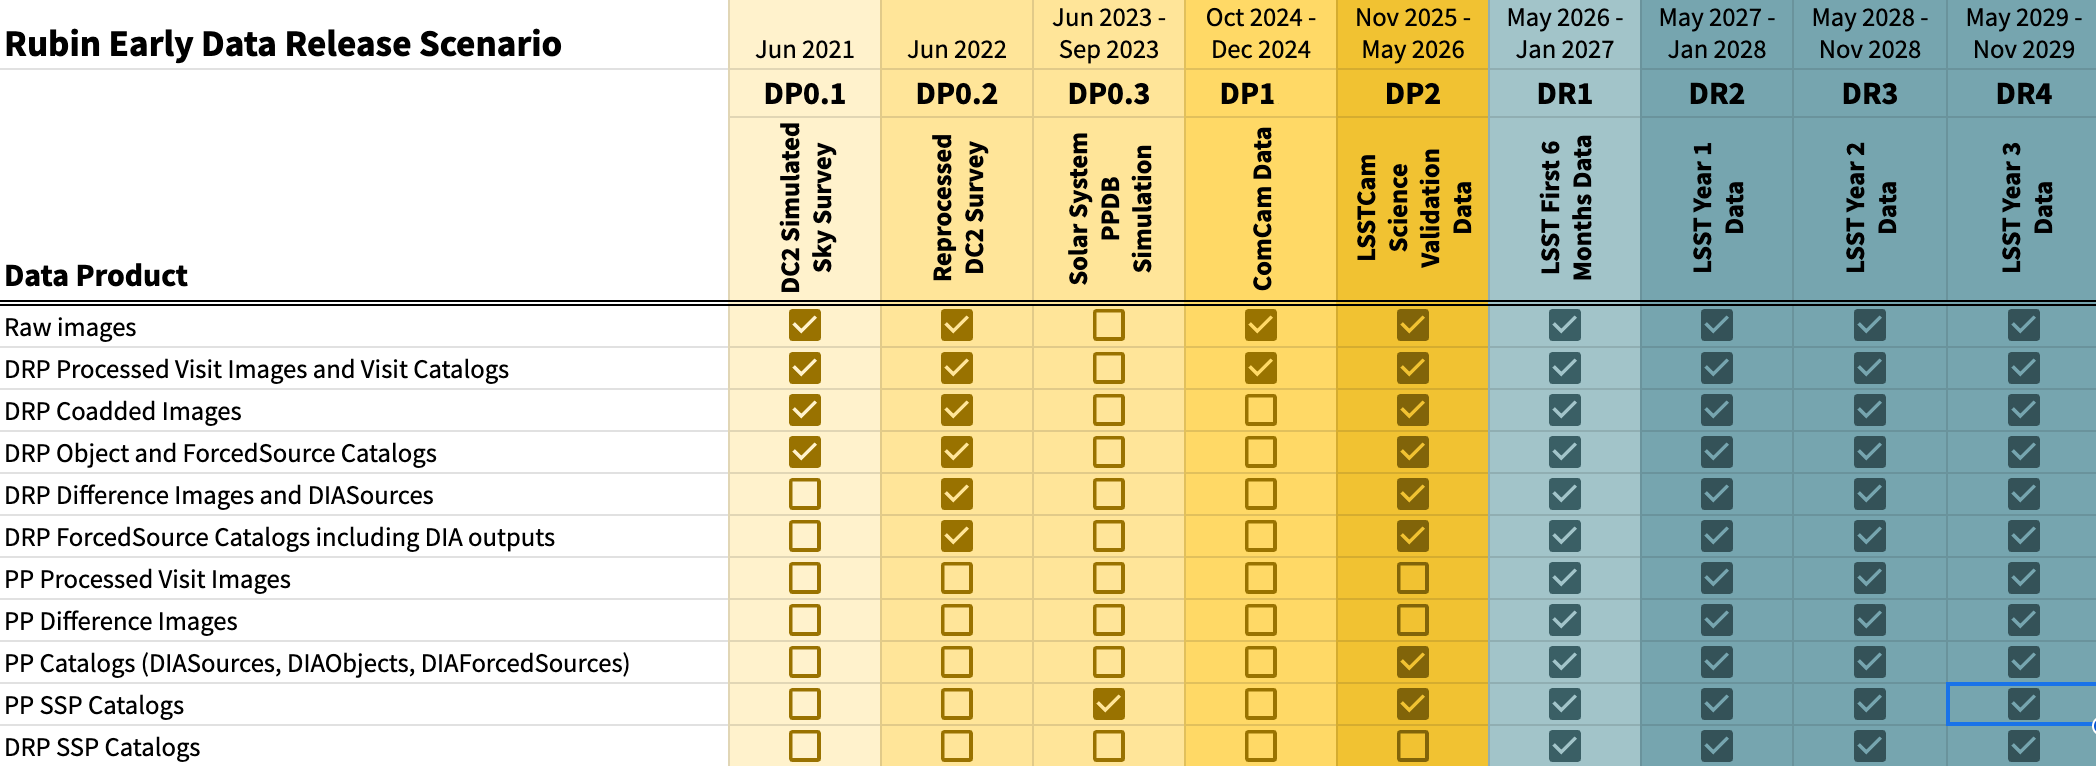
\includegraphics[width=\linewidth]{figures/DPR-summary}
\end{table}

\begin{table}
\caption{Summary of data products expected in DP1, as of October 2022.}
\label{tab:dp-one-products}
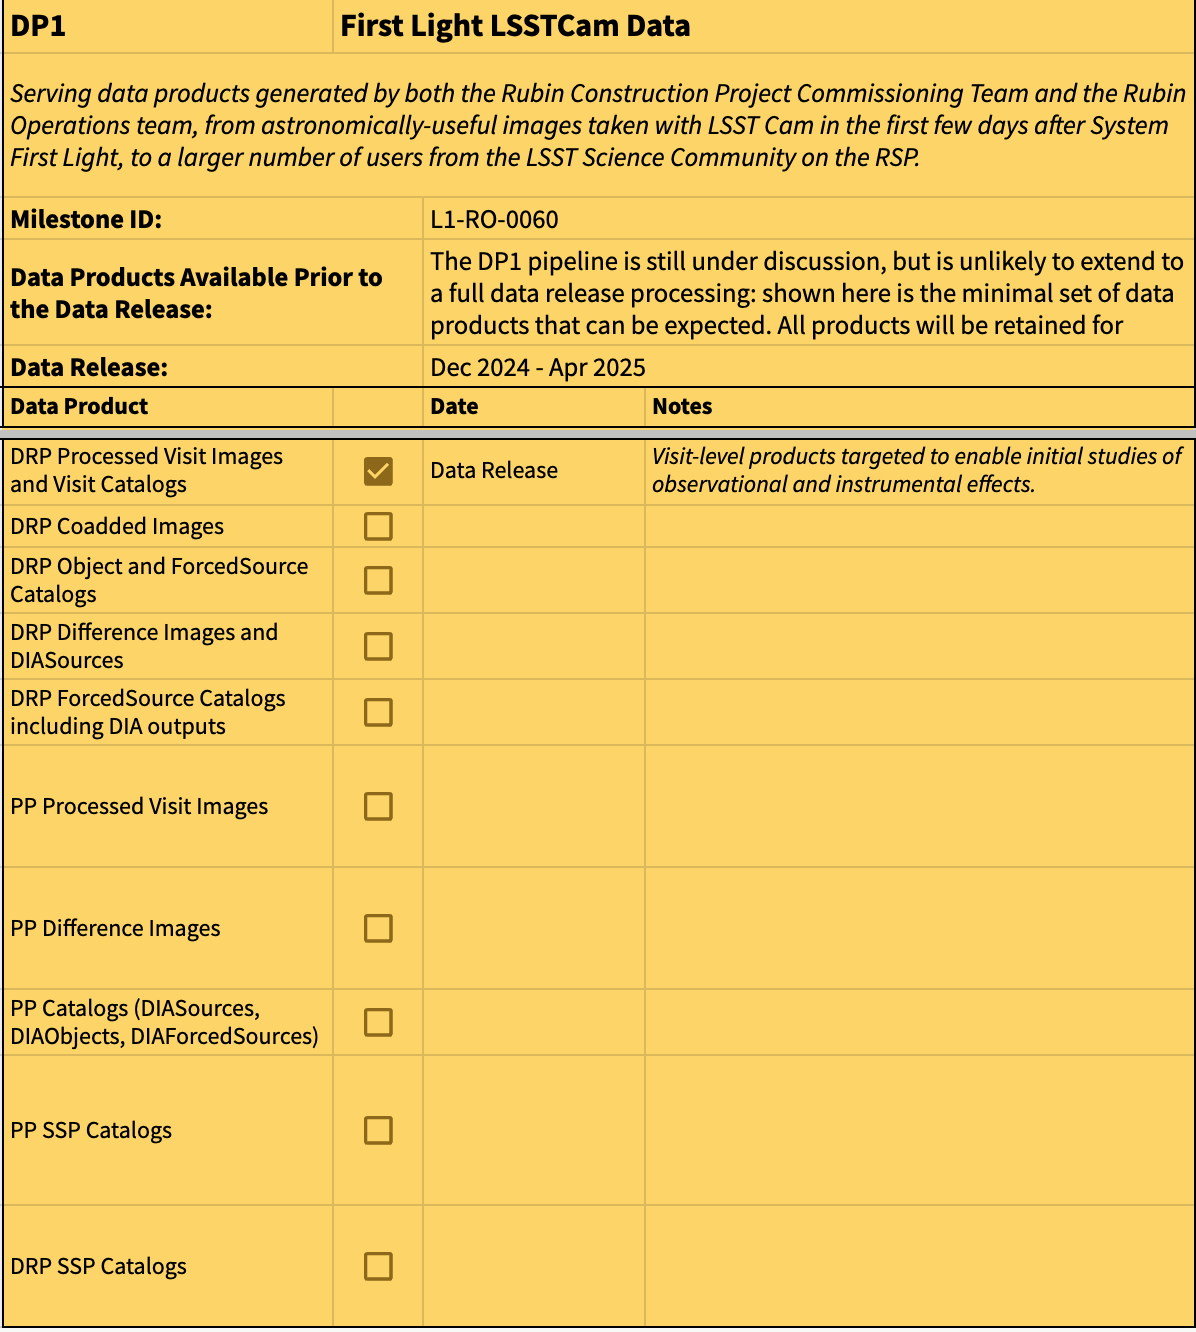
\includegraphics[width=\linewidth]{figures/DP1-products}
\end{table}

\begin{table}
\caption{Summary of data products expected in DP2, as of October 2022.}
\label{tab:dp-two-products}
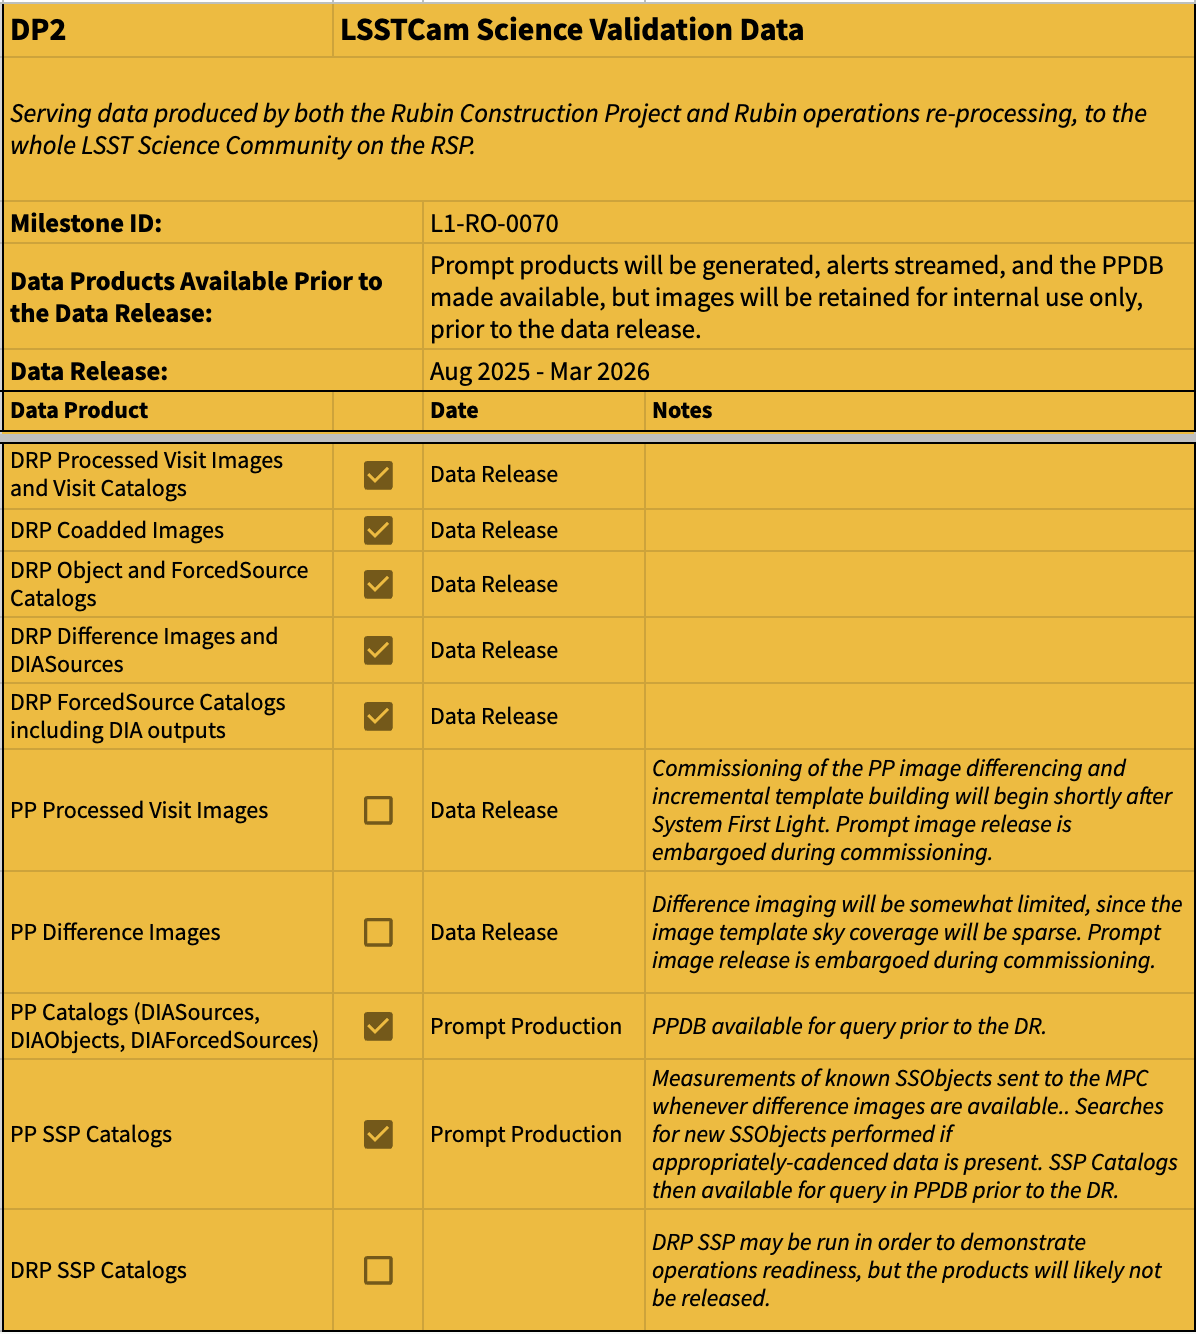
\includegraphics[width=\linewidth]{figures/DP2-products}
\end{table}

\begin{table}
\caption{Summary of data products expected in DR1, as of October 2022.}
\label{tab:dr-one-products}
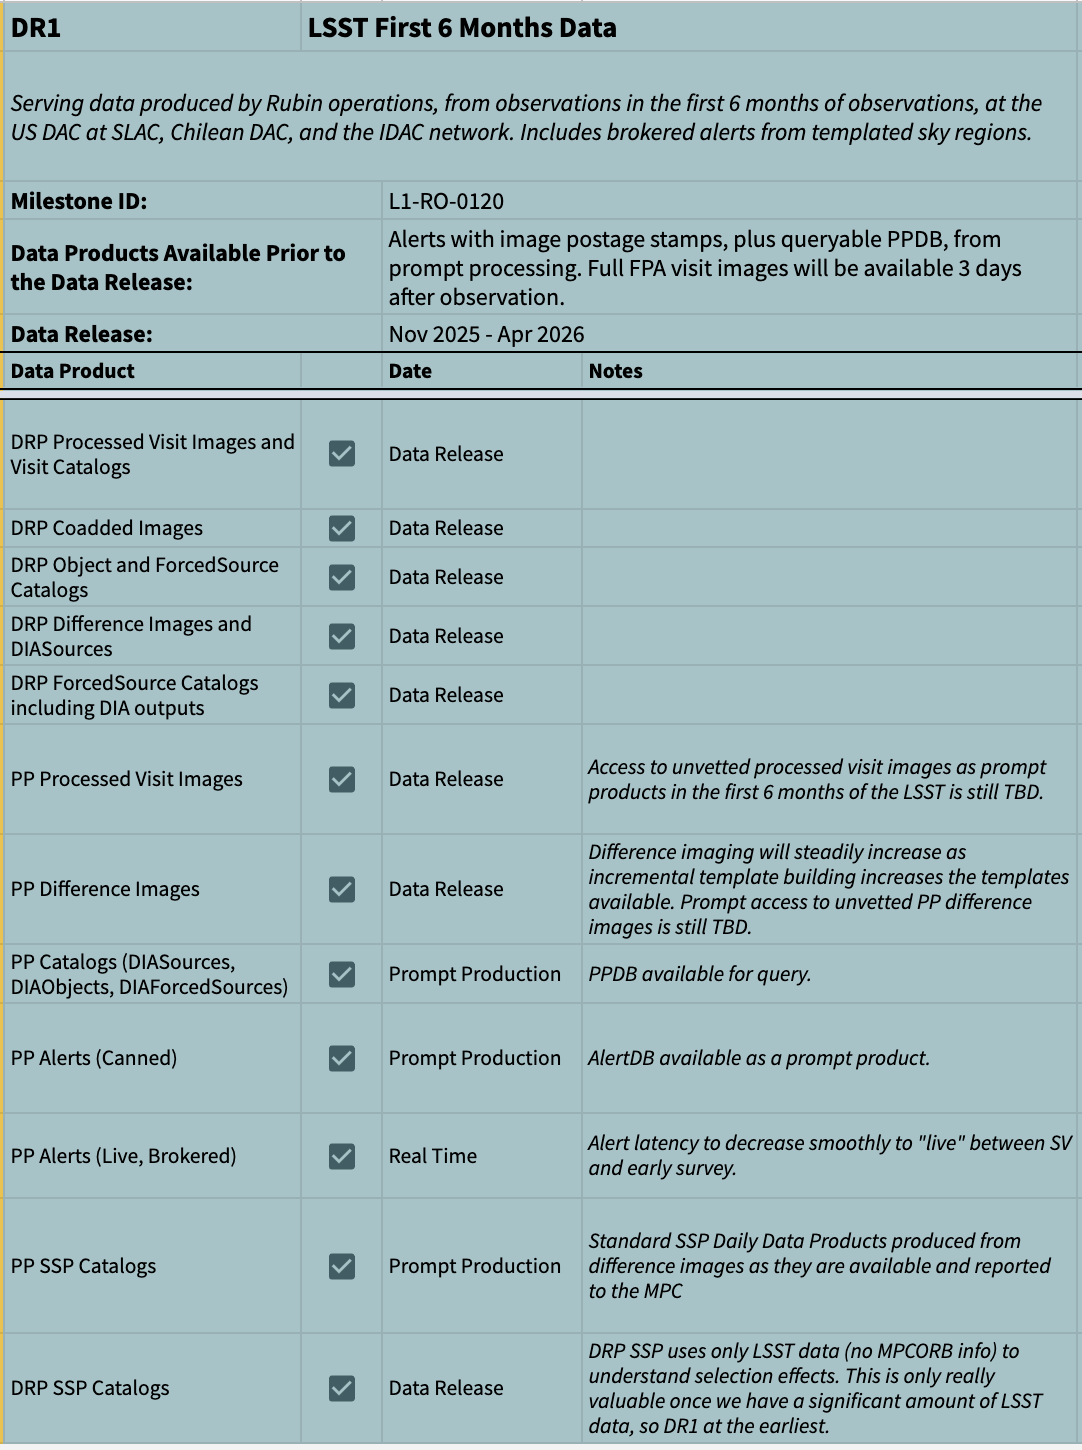
\includegraphics[width=\linewidth]{figures/DR1-products}
\end{table}
